\documentclass{article}

\usepackage{amsmath}
\usepackage{amsfonts}
\usepackage{tikz}

\usetikzlibrary{calc}
\usetikzlibrary{patterns} 
\newcommand\centerofmass{%
    \tikz[radius=0.4em] {%
        \fill (0,0) -- ++(0.4em,0) arc [start angle=0,end angle=90] -- ++(0,-0.8em) arc [start angle=270, end angle=180];%
        \draw (0,0) circle;%
    }%
}

\begin{document}

\section{Problem 7-8}

%	\begin{tikzpicture}
%	
%	\coordinate (base) at (0,0);
%	\coordinate (elbow) at (3,2);
%	\coordinate (joint-1) at (2.4453, 2.83205);
%	\coordinate (bottom-of-slider) at (1.19722, 2.0);
%	\coordinate (top-of-slider) at (4.5254, 4.2188);
%	\coordinate (base-of-arrow) at (2.889, 3.0678);
%	\coordinate (middle-of-arrow) at (2.938, 2.926);
%	\coordinate (head-of-arrow) at (3.0277, 2.859);
%	\coordinate (arrow-link-in-joint-1) at (2.5812, 2.68228);
%	
%	\draw[-] (-1,0) to (1,0);
%	\fill (base) circle (0.07);
%	\draw[-] (base) to node {\centerofmass} (elbow);
%	\draw[-] (elbow) to node {\centerofmass} (joint-1);
%	\draw[-] (top-of-slider) to node {\centerofmass} (bottom-of-slider);
%	\draw[-] (head-of-arrow) to (base-of-arrow);
%	\draw[<->] (arrow-link-in-joint-1) to node[below right] {$q_2$} (middle-of-arrow);
%	
%	\draw[<->] (0.75, 0)  node[above right] {$q_1$} arc(0:33:0.75);
%	
%	\end{tikzpicture}

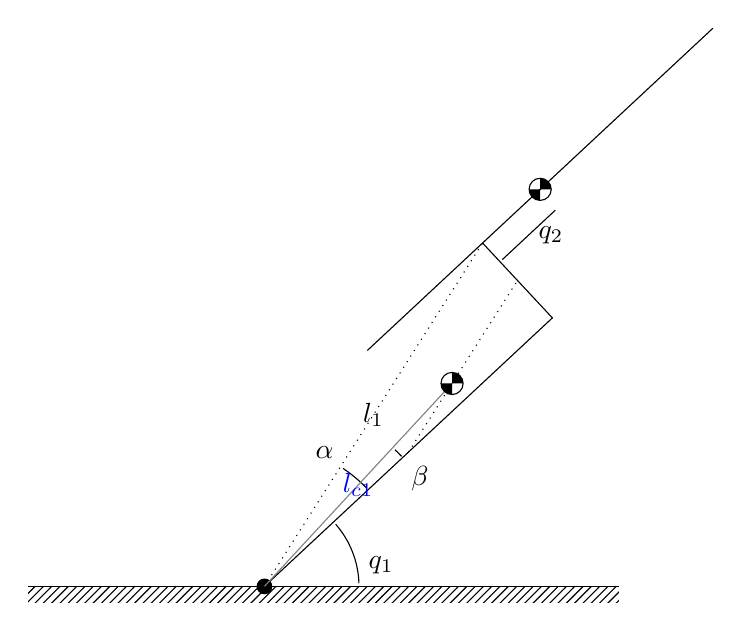
\begin{tikzpicture}[scale=2.0]
%VARIABLES
%%%%%%%%%%%%%%%%%%%%

% model parameters
\def \loneone {2.5};
\def \lconeone {0.5*\loneone};
\def \lonetwo {0.65};
\def \lconetwo {0.5*\lonetwo};
\def \ltwo {3.0};
\def \lctwo {1.5};
\def \moneone {0.3};
\def \monetwo {0.2};

% joint-space
\def \qone {43.0};
\def \qtwo {0.5};

% drawing parameters
% q1 angle drawing
\def \angleconedist {0.6};
\def \angleconeoffset { 0.02 };
\def \angleconeradius {sqrt( \angleconedist*\angleconedist + \angleconeoffset*\angleconeoffset)};
\def \angleconestartangle { atan2( \angleconeoffset, \angleconedist)};
\def \angleconeendangle { \qone - \angleconestartangle};
% alpha angle drawing
\def \alphaangleconedist {0.9};
\def \alphaangleconeoffset { 0.02 };
\def \alphaangleconeradius {sqrt( \alphaangleconedist*\alphaangleconedist + \alphaangleconeoffset*\alphaangleconeoffset)};
\def \alphaangleconestartangle { \qone + atan2( \alphaangleconeoffset, \alphaangleconedist)};
\def \alphaangleconeendangle { \qone + atan2(\lonetwo, \loneone) - atan2( \alphaangleconeoffset, \alphaangleconedist)};
% beta angle drawing
\def \anglebeta {atan2((\monetwo/(\moneone+\monetwo))*\lconetwo,(1 + \moneone/(\moneone+\monetwo))*\lconeone)};
\def \betaangleconedist {1.2};
\def \betaangleconeoffset { 0.01 };
\def \betaangleconeradius {sqrt( \betaangleconedist*\betaangleconedist + \betaangleconeoffset*\betaangleconeoffset)};
\def \betaangleconestartangle { \qone + atan2( \betaangleconeoffset, \betaangleconedist)};
\def \betaangleconeendangle { \qone + \anglebeta - atan2( \betaangleconeoffset, \betaangleconedist)};
% floor dimensions
\def \leftfloorextent { 1.5};
\def \rightfloorextent {2.25};

\def \arrowoffset {0.25*\lonetwo};
\def \arrowmargin {0.02};

% COORDINATES
%%%%%%%%%%%%%%%%%%%%%%
\coordinate (arm-1-1-normal) at ({cos(\qone)}, {sin(\qone)});
\coordinate (arm-1-2-normal) at ({-sin(\qone)}, {cos(\qone)});

% ground
\coordinate (base-point) at (0,0);
\coordinate (left-ground) at ({-\leftfloorextent}, 0);
\coordinate (right-ground) at ({\rightfloorextent}, 0);
\coordinate (right-underground) at ($(right-ground) - (0.0, 0.1)$);

\coordinate (arm-elbow-1) at ($ (base-point) + \loneone*(arm-1-1-normal) $);
\coordinate (arm-cm-1) at ($ (base-point) + \lconeone*(arm-1-1-normal) $);
\coordinate (arm-end-1) at ($ (arm-elbow-1) + \lonetwo*(arm-1-2-normal) $);
\coordinate (arm-cm-2) at ($ (arm-elbow-1) + \lconetwo*(arm-1-2-normal) $);
\coordinate (arm-cm) at ($ (base-point) + {\moneone/(\moneone + \monetwo)}*(arm-cm-1) 
	+ {\monetwo/(\moneone + \monetwo)}*(arm-cm-2) $);
\coordinate (slider-rear) at ($ (arm-end-1) + {\qtwo - \lctwo}*(arm-1-1-normal) $);
\coordinate (slider-front) at ($ (arm-end-1) + {\lctwo + \qtwo}*(arm-1-1-normal) $);
\coordinate (slider-cm) at ($(arm-end-1) + \qtwo*(arm-1-1-normal)$);



% DRAWINGS

% ground
\draw (left-ground) -- (right-ground);
\fill[pattern = north east lines] (left-ground) rectangle (right-underground);

% arm part 1
\fill (base-point) circle (0.05);
\draw (base-point) -- (arm-elbow-1) -- (arm-end-1);
\draw[dotted] (base-point) -- node {$l_1$}(arm-end-1);
\draw[dotted] (arm-cm-1) -- (arm-cm-2);
\draw ($ (base-point) + (\angleconedist, \angleconeoffset)$) node[above right] {$q_1$} 
	arc ({\angleconestartangle}:{\angleconeendangle}:{\angleconeradius});
\draw ($ (base-point) + \alphaangleconedist*(arm-1-1-normal) + \alphaangleconeoffset*(arm-1-2-normal)$) 
	arc ({\alphaangleconestartangle}:{\alphaangleconeendangle}:{\alphaangleconeradius})
	node[above left] {$\alpha$};
\draw ($ (base-point) + \betaangleconedist*(arm-1-1-normal) + \betaangleconeoffset*(arm-1-2-normal)$) 
	node[below right] {$\beta$}
	arc ({\betaangleconestartangle}:{\betaangleconeendangle}:{\betaangleconeradius});
\draw[color=gray] (base-point) -- node[color=blue] {$l_{c1}$}(arm-cm);

% arm part 2
\draw (slider-rear) -- (arm-end-1) -- (slider-front);
\draw ($ (arm-end-1) - \arrowoffset*(arm-1-2-normal) + \arrowmargin*(arm-1-1-normal)$) 
	to node[right] {$q_2$} ($ (slider-cm) - \arrowoffset*(arm-1-2-normal) - \arrowmargin*(arm-1-1-normal)$);

\node at (arm-cm) {\centerofmass};
\node at (slider-cm) {\centerofmass};

\end{tikzpicture}


\paragraph{}
We will first determine the velocity jacobians for the first two centers of mass.
The vector from the origin to the first center of mass is:

\begin{align*}
o_{c1} & = \left[ \begin{matrix} l_{c1} \cos (q_1 + \beta) \\ l_{c1}\sin (q_1 + \beta) \\ 0 \end{matrix} \right]
\end{align*}

Since the first joint is along the $z$ axis, the jacobian for the first center of mass is:

\begin{align}
J_1 & = \left[ \begin{matrix}
	- l_{c1} \sin (q_1 + \beta) & 0 \\
	l_{c1} \cos (q_1 + \beta) & 0 \\
	0 & 0 \\
	\end{matrix} \right]
\end{align}

For the first column of the second velocity jacobian, we can compute the vector to the center of mass:

\begin{align*}
o_{c2} & = \left[ \begin{matrix} 
	l_1 \cos (q_1 + \alpha) + q_2 \cos q_1 \\ 
	l_1 \sin (q_1 + \alpha) + q_2 \sin q_1 \\
	0 \\
	\end{matrix} \right]
\end{align*}

Therefore, the jacobian at the center of mass is given by:

\begin{align}
J_2 & = \left[ \begin{matrix}
	- l_1 \sin (q_1 + \alpha) - q_2 \sin q_1 & \cos q_1 \\
	l_1 \cos (q_1 + \alpha) + q_2 \cos q_1 & \sin q_1 \\ 
	0 & 0 \\
	\end{matrix} \right]
\end{align}

The angular velocities of both arms are $\dot{q_1}$, so if $I_1$ is the moment of inertia
	of part 1 about its center of mass, and $I_2$ is the moment of inertia of part 2 about
	its center of mass, the total kinetic energy is given by:

\begin{align}
	T & = \frac 1 2 \dot{q}^T D(q) \dot{q}\\
	D(q) & = \left[ \begin{matrix}
		m_1 l_{c1}^2 + m_2 \left( l_1^2 + 2 l_1 q_2 + q_2^2 \right) + I_1 + I_2 
		& - m_2 l_1 \sin \alpha \\
		- m_2 l_1 \sin \alpha & m_2 \\
	\end{matrix} \right]
\end{align}

Now that we have $D(q)$, we can compute the Christoffel Symbols:

\begin{align}
c_{111} & = \frac 12 \frac {\partial d_{11}}{\partial q_1} = 0 \\
c_{121} & = c_{211} = \frac 1 2 \frac {\partial d_{11}}{\partial q_2} = m_2 \left( l_1 + q_2 \right) \\
c_{221} & = \frac {\partial d_{12}}{\partial q_2} - \frac 12 \frac {\partial d_{22}}{\partial q_1}
	= 0 \\ 
c_{112} & = \frac {\partial d_{21}}{\partial q_1} - \frac 12 \frac {\partial d_{11}}{\partial q_2}
	=  - m_2 \left( l_1 + q_2 \right) \\ 
c_{212} & = c_{122} = \frac 12 \frac {\partial d_{22}}{\partial q_1} = 0 \\
c_{222} & = \frac 12 \frac{\partial d_{22}}{\partial q_2} = 0
\end{align}

The gravitational potential energy is given by:

\begin{align}
P(q) & = g \left( m_1 l_{c1} \sin (q_1 + \beta)   + m_2 \left( l_1 \sin (q_1 + \alpha) + q_2 \sin (q_1) \right) \right)
\end{align}

Therefore, the euler-lagrange equations can be written:

\begin{align}
\left( m_1 l_{c1}^2 + m_2 \left( l_1^2 + 2 l_1 q_2 + q_2^2 \right) + I_1 + I_2 \right)
\ddot{q_1}
- m_2 l_1 \sin \alpha \ddot{q_2} \nonumber \\
+ m_2 (l_1 + q_2) \dot{q_1} \dot{q_2} + \nonumber \\
g \left( m_1 l_{c1} \cos (q_1 + \beta) + m_2 \left( l_1 \cos (q_1 + \alpha) + q_2 \cos (q_1) \right) \right)
& = \tau_1 \\
m_2 l_1 \sin \alpha \ddot{q_1}
+ m_2 \ddot{q_2} + m_2 l_1 \sin \alpha \dot{q_1} \dot{q_2} +
g m_2 \cos (q_1)
& = \tau_2 
\end{align}

\section{Moment Labeling}

\subsection{Example 1}

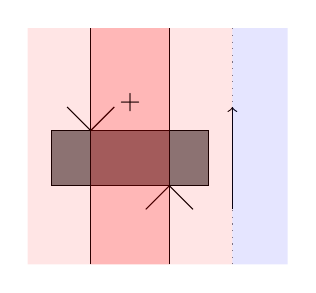
\begin{tikzpicture}

\def \width {2.0};
\def \height {0.7};
\def \contactsize {0.3};
\def \bottominf {-1.0};
\def \topinf{2.0};
\def \leftinf{-0.3};
\def \rightinf{\width + 1.0};

\def \sideoffset {0.5};

\fill[color=gray] (0,0) -- ({\width},0) -- ({\width},{\height}) -- (0,{\height}) -- (0,0);
\draw[color=black] (0,0) -- ({\width},0) -- ({\width},{\height}) -- (0,{\height}) -- (0,0);

\draw ({\sideoffset - \contactsize},{\contactsize + \height}) -- ({\sideoffset},{\height}) -- ({\sideoffset + \contactsize},{\contactsize+\height});
\draw ({\width - (\sideoffset - \contactsize)},{-\contactsize}) -- ({\width - \sideoffset},0) -- ({\width - (\sideoffset + \contactsize)},{-\contactsize});

\draw ({\sideoffset},{\bottominf}) -- ({\sideoffset},{\topinf});
\draw ({\width - \sideoffset},{\bottominf}) -- ({\width - \sideoffset},{\topinf});

\fill[color=red,opacity=0.2] ({\sideoffset},{\bottominf}) -- ({\width - \sideoffset},{\bottominf}) -- ({\width - \sideoffset},{\topinf}) -- ({\sideoffset}, {\topinf}) -- ({\sideoffset},{\bottominf});

\node at ({\width/2},{1.5*\height}) {$+$};

\draw[->] ({\width + \contactsize},{-\contactsize}) -- ({\width + \contactsize},{\height + \contactsize});
\draw[color=gray, dotted] ({\width + \contactsize},{\bottominf}) -- ({\width + \contactsize},{-\contactsize});
\draw[color=gray, dotted] ({\width + \contactsize},{\topinf}) -- ({\width + \contactsize},{\height + \contactsize});
\fill[color=red, opacity=0.1] ({\leftinf, \bottominf}) -- ({\width + \contactsize, \bottominf}) -- ({\width + \contactsize, \topinf}) -- ({\leftinf, \topinf}) -- ({\leftinf, \bottominf});
\fill[color=blue, opacity=0.1] ({\rightinf, \bottominf}) -- ({\width + \contactsize, \bottominf}) -- ({\width + \contactsize, \topinf}) -- ({\rightinf, \topinf}) -- ({\rightinf, \bottominf});
\end{tikzpicture}

\subsection{b}

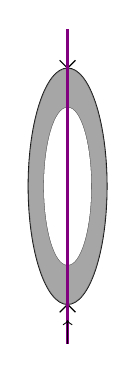
\begin{tikzpicture}

\def \bottominf {-2.0};
\def \topinf {2.0};

\draw (0,0) ellipse (0.5 and 1.5);
\draw (0,0) ellipse (0.3 and 1.0);
\fill[color=gray, opacity= 0.7] (0,0) ellipse (0.5 and 1.5);
\fill[color=white] (0,0) ellipse (0.3 and 1.0);

\draw (-0.1, 1.6) -- (0.0, 1.5) -- (0.1, 1.6);
\draw (-0.1, -1.6) -- (0.0, -1.5) -- (0.1, -1.6);

\draw[color=violet, thick] (0.0, \bottominf) -- (0.0, \topinf);

\draw[->] (0.0, \bottominf) -- (0.0, -1.7);

\end{tikzpicture}

The object can only resist wrenches applied in either direction along
	the purple line.
If the objects is pushed from either side, the unstable local minima will
	slip from the points and the shape will be lost.

\subsection{c}

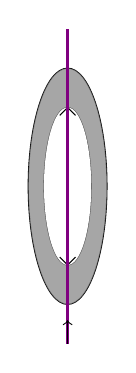
\begin{tikzpicture}

\def \bottominf {-2.0};
\def \topinf {2.0};

\draw (0,0) ellipse (0.5 and 1.5);
\draw (0,0) ellipse (0.3 and 1.0);
\fill[color=gray, opacity= 0.7] (0,0) ellipse (0.5 and 1.5);
\fill[color=white] (0,0) ellipse (0.3 and 1.0);

\draw (-0.1, 0.9) -- (0.0, 1.0) -- (0.1, 0.9);
\draw (-0.1, -0.9) -- (0.0, -1.0) -- (0.1, -0.9);

\draw[color=violet, thick] (0.0, \bottominf) -- (0.0, \topinf);

\draw[->] (0.0, \bottominf) -- (0.0, -1.7);

\end{tikzpicture}

This object can only resist wrenches applied in either direction along
	the line, in the first order labeling.
Unlike the previous section, however, a small rotation will result in a normal
	force, and any translation will also result in a normal force,
	because both contacts are local maxima in the shape.

\subsection{d}

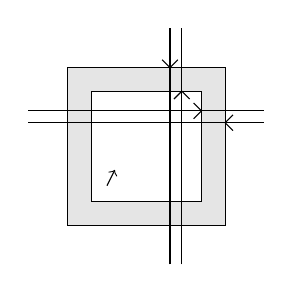
\begin{tikzpicture}

\def \width {2.0};
\def \height {2.0};
\def \thick {0.3};
\def \leftend {-0.5};
\def \rightend {2.5};
\def \bottomend {-0.5}
\def \topend{2.5};

\draw[fill=gray!20] (0,0) rectangle ({\width}, {\height});
\draw[fill=white] (\thick,\thick) rectangle ({\width-\thick},{\height-\thick});

\draw (1.2, 2.1) -- (1.3,2.0) -- (1.4,2.1);
\draw (1.3,\bottomend) -- (1.3, \topend);
\draw (1.35, 1.6) -- (1.45, 1.7) -- (1.55, 1.6);
\draw (1.45,\bottomend) -- (1.45, \topend);
\draw (1.6, 1.35) -- (1.7, 1.45) -- (1.6, 1.55);
\draw (\leftend, 1.45) -- (\rightend, 1.45);
\draw (2.1, 1.2) -- (2.0,1.3) -- (2.1,1.4);
\draw (\leftend, 1.3) -- (\rightend, 1.3);

\draw[->] (0.5, 0.5) -- (0.6, 0.7);

\end{tikzpicture}

\paragraph{}
This object is entirely attached: there are no limits on the resultant
	wrenches it can call upon to resist an applied wrench.
No point is to the left of all of the lines of force, or to the right
	of all of them.

\subsection{e}

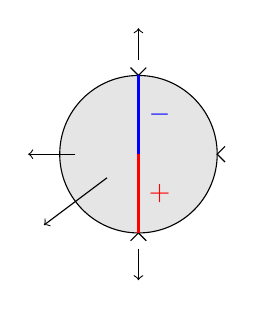
\begin{tikzpicture}

\draw[fill=gray!20] (0,0) circle (1.0);
\draw (-0.1, 1.1) -- (0, 1) -- (0.1, 1.1);
\draw (-0.1, -1.1) -- (0, -1) -- (0.1, -1.1);
\draw (1.1, 0.1) -- (1, 0) -- (1.1, -0.1);

\draw[color=red, thick] (0,-1) -- node[right] {$+$} (0,0);
\draw[color=blue, thick] (0,0) -- node[right] {$-$} (0,1);

\draw[->] (-0.8, 0) -- (-1.4, 0);
\draw[->] (0.0, 1.2) -- (0.0, 1.6);
\draw[->] (0.0, -1.2) -- (0.0, -1.6);
\draw[->] (-0.4, -0.3) -- (-1.2, -0.9);

\end{tikzpicture}

This sphere can only create resultant forces which place the red 
	region entirely on the left, and the blue region entirely along
	the right, or are on that line exactly.
Therefore the possible resultant forces are only ones which emenate from the
	center of the sphere, and are going leftwards.

\subsection{f}

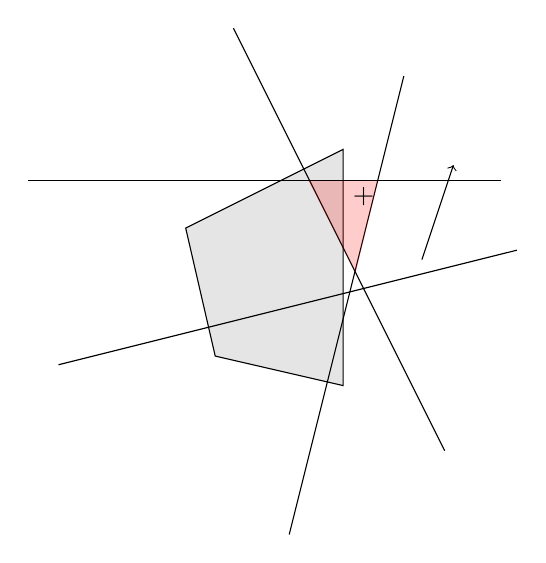
\begin{tikzpicture}[scale=2.0]

\coordinate (point1) at (0,1);
\coordinate (point2) at (0.1875, 0.1875);
\coordinate (point3) at (1,0);
\coordinate (point4) at (1,1.5);

\coordinate (joint1) at (0.9, 0.025);
\coordinate (joint1parallel) at ({cos(atan2(-0.25,1.0))},{sin(atan2(-0.25,1.0))});
\coordinate (joint1normal) at ({cos(90 + atan2(-0.25,1.0))},{sin(90 + atan2(-0.25,1.0))});

\coordinate (joint2) at (0.1625, 0.375);
\coordinate (joint2normal) at ({cos(atan2(0.25, 1.0))},{sin(atan2(0.25, 1.0))});

\coordinate (joint3) at (0.75, 1.375);
\coordinate (joint3normal) at ({cos(atan2(-1.0, 0.5))},{sin(atan2(-1.0, 0.5))});

\coordinate (joint4) at (1.0, 1.3);
\coordinate (joint4normal) at (-1.0, 0.0);

\draw[fill=gray!20] (point1) -- (point2) -- (point3) -- (point4) -- cycle;
\draw ($ (joint1) - (joint1normal) $) -- ($ (joint1) + 2*(joint1normal) $);
\draw ($ (joint2) - (joint2normal) $) -- ($ (joint2) + 2*(joint2normal) $);
\draw ($ (joint3) - (joint3normal) $) -- ($ (joint3) + 2*(joint3normal) $);
\draw ($ (joint4) - (joint4normal) $) -- ($ (joint4) + 2*(joint4normal) $);

\fill[color=red,opacity=0.2] (1.08, 0.72) -- (1.22, 1.3) -- (0.78, 1.3) -- cycle;

\node[right] at (1.0, 1.2) {$+$};

\draw[->] (1.5, 0.8) -- (1.7, 1.4);

\end{tikzpicture}

This shape can supply most resultant wrenches, but it cannot resist some
	rotations.
Once any wrench moves the object a small amount, however, second-order
	effects will prevent the object from being turned, becuase it is held
	rigidly on all sides with flat surfaces.

\section{Grasp Types}

\begin{tabular}{l | l | l | l | l }
Body & First-Order Form Closure & Second-Order Form Closure & Caged & Force Closure\\
\hline
a & No & No & No & No \\
b & No & No & No & No \\
c & No & Yes & No & No (curved contacts) \\
d & Yes & Yes & Yes & Yes\\
e & No & No & No & No\\
f & No & Yes & Yes & Yes \\
\end{tabular}

\section{Tipping Rectangle}

Consider the rectangle in the following picture:

\paragraph{}
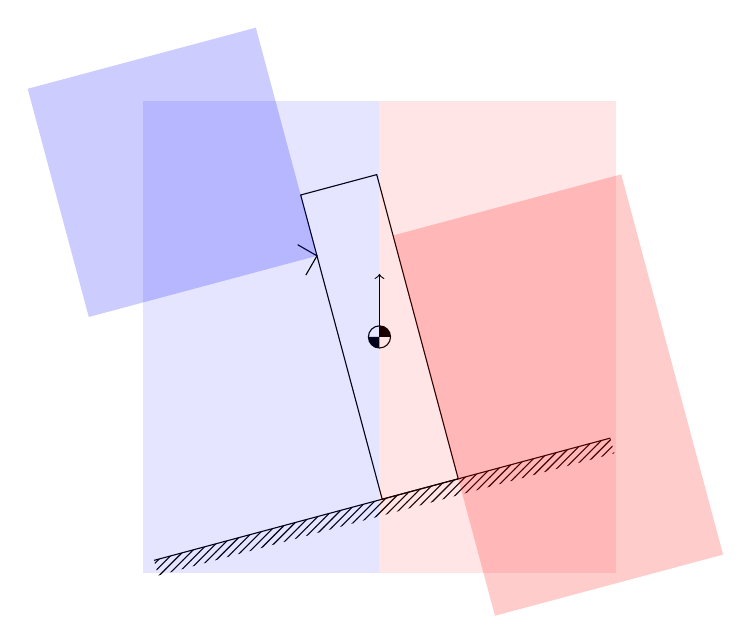
\begin{tikzpicture}[scale=2.0]
% VARIABLES 
%%%%%%%%%%%%%%%%%%%%%
\def \width {0.5};
\def \height {2.0};
\def \slopelength {3.0};
\def \rectanglepositiononslope {1.5};
\def \slopeangle {15};
\def \crosshatchdepth {0.1};
\def \fingerfraction {0.8};
\def \fingerheight {\fingerfraction*\height};
\def \fingersize {0.1};
\def \bottominf {-0.5};
\def \topinf {3.0};

% COORDINATES 
%%%%%%%%%%%%%%%%%%%%
% coordinate system
\coordinate (rectangle-base-vector) at ({cos(\slopeangle)}, {sin(\slopeangle)});
\coordinate (rectangle-side-vector) at ({-sin(\slopeangle)}, {cos(\slopeangle)});

% slope
\coordinate (base-of-slope) at (0,0);
\coordinate (top-of-slope) at ($ \slopelength*(rectangle-base-vector) $);

% shading
\coordinate (bottom-left-shading) at ($ (base-of-slope) - \crosshatchdepth*(rectangle-side-vector)$);
\coordinate (bottom-right-shading) at ($ (top-of-slope) - \crosshatchdepth*(rectangle-side-vector)$);

% rectangle
\coordinate (bottom-left-rectangle) at ($ \rectanglepositiononslope*(rectangle-base-vector) $);
\coordinate (bottom-right-rectangle) at ($ (bottom-left-rectangle) + \width*(rectangle-base-vector) $);
\coordinate (top-left-rectangle) at ($ (bottom-left-rectangle) + \height*(rectangle-side-vector) $);
\coordinate (top-right-rectangle) at ($ (bottom-right-rectangle) + \height*(rectangle-side-vector) $);
\coordinate (center-of-mass) at ($ (bottom-left-rectangle) + 0.5*\width*(rectangle-base-vector) + 0.5*\height*(rectangle-side-vector)$);
\coordinate (finger) at ($ (bottom-left-rectangle) + \fingerheight*(rectangle-side-vector)$);
\coordinate (fingerotherside) at ($ (bottom-left-rectangle) + \fingerheight*(rectangle-side-vector) + \width*(rectangle-base-vector)$);

% DRAWING
%%%%%%%%%%%%%%%%%%

% slope
\draw[solid] (base-of-slope) -- (top-of-slope);

% shading
\fill[pattern=north east lines, pattern color=black] (base-of-slope) -- (top-of-slope)
                                                                     -- (bottom-right-shading)
                                                                     -- (bottom-left-shading)
                                                                     -- (base-of-slope);

% rectangle
\draw (bottom-left-rectangle) -- (bottom-right-rectangle)
                              -- (top-right-rectangle)
                              -- (top-left-rectangle)
                              -- (bottom-left-rectangle);
\node at (center-of-mass) {\centerofmass};
\fill[color=blue, opacity=0.1] ($ (center-of-mass) + (0, -1.5)$)
	-- ($ (center-of-mass) + (0, 1.5)$)
	-- ($ (center-of-mass) + (-1.5, 1.5)$)
	-- ($ (center-of-mass) + (-1.5, -1.5)$)
	-- cycle;
\fill[color=red, opacity=0.1] ($ (center-of-mass) + (0, -1.5)$)
	-- ($ (center-of-mass) + (0, 1.5)$)
	-- ($ (center-of-mass) + (1.5, 1.5)$)
	-- ($ (center-of-mass) + (1.5, -1.5)$)
	-- cycle;
\draw[->] (center-of-mass) -- ($ (center-of-mass) + (0,0.4)$);
% rectangle cross hatches

% finger
\draw ($(finger) - \fingersize*(rectangle-base-vector) + \fingersize*(rectangle-side-vector)$)
	-- (finger)
	-- ($(finger) - \fingersize*(rectangle-base-vector) - \fingersize*(rectangle-side-vector)$);

\fill[color=blue, opacity=0.2] (finger)
	-- ($ (finger) + 1.5*(rectangle-side-vector)$)
	-- ($ (finger) + 1.5*(rectangle-side-vector) - 1.5*(rectangle-base-vector)$)
	-- ($ (finger) - 1.5*(rectangle-base-vector)$)
	-- cycle;

\fill[color=red, opacity=0.2] (fingerotherside)
	-- ($ (fingerotherside) - 2.5*(rectangle-side-vector)$)
	-- ($ (fingerotherside) - 2.5*(rectangle-side-vector) + 1.5*(rectangle-base-vector)$)
	-- ($ (fingerotherside) + 1.5*(rectangle-base-vector)$)
	-- cycle;
\end{tikzpicture}

We will first determine if there is a static equilibrium.
In this case, a resultant wrench, emenating from the center of mass and going 
	directly upwards, as shown in the above figure, is compatible
	with the constraints.
Therefore, in this configuration, the block can resist the external force
	from gravity.

However, if we tilt more and move the contact point up slightly:

\paragraph{}
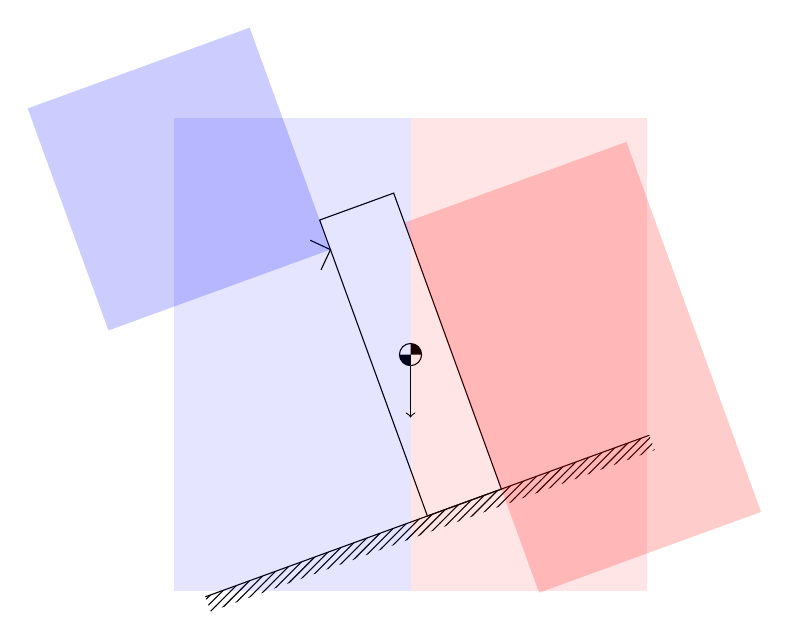
\begin{tikzpicture}[scale=2.0]
% VARIABLES 
%%%%%%%%%%%%%%%%%%%%%
\def \width {0.5};
\def \height {2.0};
\def \slopelength {3.0};
\def \rectanglepositiononslope {1.5};
\def \slopeangle {20};
\def \crosshatchdepth {0.1};
\def \fingerfraction {0.9};
\def \fingerheight {\fingerfraction*\height};
\def \fingersize {0.1};
\def \bottominf {-0.5};
\def \topinf {3.0};

% COORDINATES 
%%%%%%%%%%%%%%%%%%%%
% coordinate system
\coordinate (rectangle-base-vector) at ({cos(\slopeangle)}, {sin(\slopeangle)});
\coordinate (rectangle-side-vector) at ({-sin(\slopeangle)}, {cos(\slopeangle)});

% slope
\coordinate (base-of-slope) at (0,0);
\coordinate (top-of-slope) at ($ \slopelength*(rectangle-base-vector) $);

% shading
\coordinate (bottom-left-shading) at ($ (base-of-slope) - \crosshatchdepth*(rectangle-side-vector)$);
\coordinate (bottom-right-shading) at ($ (top-of-slope) - \crosshatchdepth*(rectangle-side-vector)$);

% rectangle
\coordinate (bottom-left-rectangle) at ($ \rectanglepositiononslope*(rectangle-base-vector) $);
\coordinate (bottom-right-rectangle) at ($ (bottom-left-rectangle) + \width*(rectangle-base-vector) $);
\coordinate (top-left-rectangle) at ($ (bottom-left-rectangle) + \height*(rectangle-side-vector) $);
\coordinate (top-right-rectangle) at ($ (bottom-right-rectangle) + \height*(rectangle-side-vector) $);
\coordinate (center-of-mass) at ($ (bottom-left-rectangle) + 0.5*\width*(rectangle-base-vector) + 0.5*\height*(rectangle-side-vector)$);
\coordinate (finger) at ($ (bottom-left-rectangle) + \fingerheight*(rectangle-side-vector)$);
\coordinate (fingerotherside) at ($ (bottom-left-rectangle) + \fingerheight*(rectangle-side-vector) + \width*(rectangle-base-vector)$);

% DRAWING
%%%%%%%%%%%%%%%%%%

% slope
\draw[solid] (base-of-slope) -- (top-of-slope);

% shading
\fill[pattern=north east lines, pattern color=black] (base-of-slope) -- (top-of-slope)
                                                                     -- (bottom-right-shading)
                                                                     -- (bottom-left-shading)
                                                                     -- (base-of-slope);

% rectangle
\draw (bottom-left-rectangle) -- (bottom-right-rectangle)
                              -- (top-right-rectangle)
                              -- (top-left-rectangle)
                              -- (bottom-left-rectangle);
\node at (center-of-mass) {\centerofmass};
\fill[color=blue, opacity=0.1] ($ (center-of-mass) + (0, -1.5)$)
	-- ($ (center-of-mass) + (0, 1.5)$)
	-- ($ (center-of-mass) + (-1.5, 1.5)$)
	-- ($ (center-of-mass) + (-1.5, -1.5)$)
	-- cycle;
\fill[color=red, opacity=0.1] ($ (center-of-mass) + (0, -1.5)$)
	-- ($ (center-of-mass) + (0, 1.5)$)
	-- ($ (center-of-mass) + (1.5, 1.5)$)
	-- ($ (center-of-mass) + (1.5, -1.5)$)
	-- cycle;
\draw[->] (center-of-mass) -- ($ (center-of-mass) - (0,0.4)$);
% rectangle cross hatches

% finger
\draw ($(finger) - \fingersize*(rectangle-base-vector) + \fingersize*(rectangle-side-vector)$)
	-- (finger)
	-- ($(finger) - \fingersize*(rectangle-base-vector) - \fingersize*(rectangle-side-vector)$);

\fill[color=blue, opacity=0.2] (finger)
	-- ($ (finger) + 1.5*(rectangle-side-vector)$)
	-- ($ (finger) + 1.5*(rectangle-side-vector) - 1.5*(rectangle-base-vector)$)
	-- ($ (finger) - 1.5*(rectangle-base-vector)$)
	-- cycle;

\fill[color=red, opacity=0.2] (fingerotherside)
	-- ($ (fingerotherside) - 2.5*(rectangle-side-vector)$)
	-- ($ (fingerotherside) - 2.5*(rectangle-side-vector) + 1.5*(rectangle-base-vector)$)
	-- ($ (fingerotherside) + 1.5*(rectangle-base-vector)$)
	-- cycle;
\end{tikzpicture}

The red region begins to be above the center of mass.
Then, the resultant wrench starting at the center of mass and going up,
	needed to oppose gravity, cannot be applied from the contacts, and therefore
	the block will tip.

One can also achieve the same effect by moving the contact point down, so that 
	the blue region is directly under the center of mass:


\paragraph{}
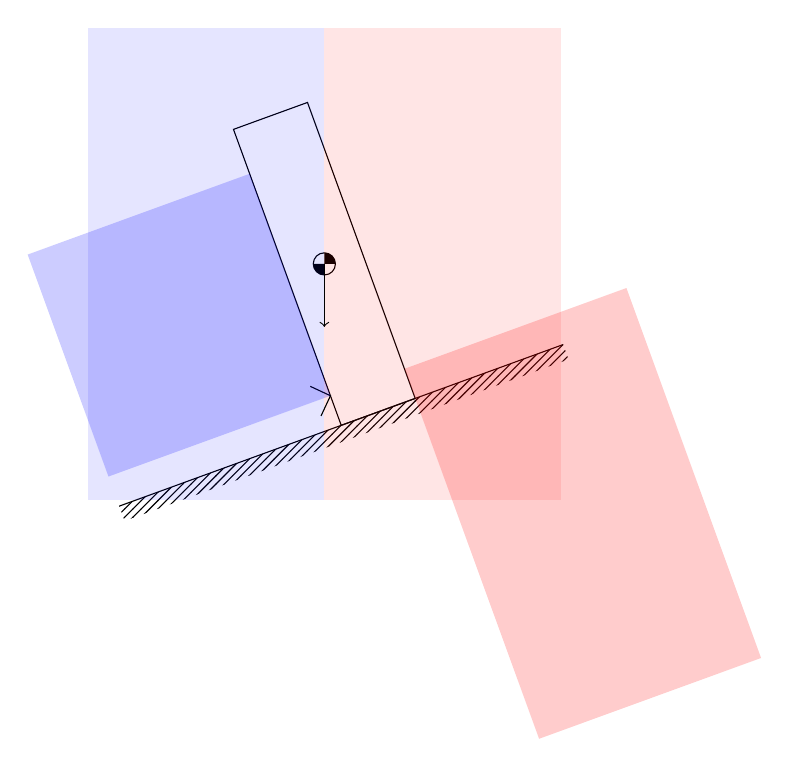
\begin{tikzpicture}[scale=2.0]
% VARIABLES 
%%%%%%%%%%%%%%%%%%%%%
\def \width {0.5};
\def \height {2.0};
\def \slopelength {3.0};
\def \rectanglepositiononslope {1.5};
\def \slopeangle {20};
\def \crosshatchdepth {0.1};
\def \fingerfraction {0.1};
\def \fingerheight {\fingerfraction*\height};
\def \fingersize {0.1};
\def \bottominf {-0.5};
\def \topinf {3.0};

% COORDINATES 
%%%%%%%%%%%%%%%%%%%%
% coordinate system
\coordinate (rectangle-base-vector) at ({cos(\slopeangle)}, {sin(\slopeangle)});
\coordinate (rectangle-side-vector) at ({-sin(\slopeangle)}, {cos(\slopeangle)});

% slope
\coordinate (base-of-slope) at (0,0);
\coordinate (top-of-slope) at ($ \slopelength*(rectangle-base-vector) $);

% shading
\coordinate (bottom-left-shading) at ($ (base-of-slope) - \crosshatchdepth*(rectangle-side-vector)$);
\coordinate (bottom-right-shading) at ($ (top-of-slope) - \crosshatchdepth*(rectangle-side-vector)$);

% rectangle
\coordinate (bottom-left-rectangle) at ($ \rectanglepositiononslope*(rectangle-base-vector) $);
\coordinate (bottom-right-rectangle) at ($ (bottom-left-rectangle) + \width*(rectangle-base-vector) $);
\coordinate (top-left-rectangle) at ($ (bottom-left-rectangle) + \height*(rectangle-side-vector) $);
\coordinate (top-right-rectangle) at ($ (bottom-right-rectangle) + \height*(rectangle-side-vector) $);
\coordinate (center-of-mass) at ($ (bottom-left-rectangle) + 0.5*\width*(rectangle-base-vector) + 0.5*\height*(rectangle-side-vector)$);
\coordinate (finger) at ($ (bottom-left-rectangle) + \fingerheight*(rectangle-side-vector)$);
\coordinate (fingerotherside) at ($ (bottom-left-rectangle) + \fingerheight*(rectangle-side-vector) + \width*(rectangle-base-vector)$);

% DRAWING
%%%%%%%%%%%%%%%%%%

% slope
\draw[solid] (base-of-slope) -- (top-of-slope);

% shading
\fill[pattern=north east lines, pattern color=black] (base-of-slope) -- (top-of-slope)
                                                                     -- (bottom-right-shading)
                                                                     -- (bottom-left-shading)
                                                                     -- (base-of-slope);

% rectangle
\draw (bottom-left-rectangle) -- (bottom-right-rectangle)
                              -- (top-right-rectangle)
                              -- (top-left-rectangle)
                              -- (bottom-left-rectangle);
\node at (center-of-mass) {\centerofmass};
\fill[color=blue, opacity=0.1] ($ (center-of-mass) + (0, -1.5)$)
	-- ($ (center-of-mass) + (0, 1.5)$)
	-- ($ (center-of-mass) + (-1.5, 1.5)$)
	-- ($ (center-of-mass) + (-1.5, -1.5)$)
	-- cycle;
\fill[color=red, opacity=0.1] ($ (center-of-mass) + (0, -1.5)$)
	-- ($ (center-of-mass) + (0, 1.5)$)
	-- ($ (center-of-mass) + (1.5, 1.5)$)
	-- ($ (center-of-mass) + (1.5, -1.5)$)
	-- cycle;
\draw[->] (center-of-mass) -- ($ (center-of-mass) - (0,0.4)$);
% rectangle cross hatches

% finger
\draw ($(finger) - \fingersize*(rectangle-base-vector) + \fingersize*(rectangle-side-vector)$)
	-- (finger)
	-- ($(finger) - \fingersize*(rectangle-base-vector) - \fingersize*(rectangle-side-vector)$);

\fill[color=blue, opacity=0.2] (finger)
	-- ($ (finger) + 1.5*(rectangle-side-vector)$)
	-- ($ (finger) + 1.5*(rectangle-side-vector) - 1.5*(rectangle-base-vector)$)
	-- ($ (finger) - 1.5*(rectangle-base-vector)$)
	-- cycle;

\fill[color=red, opacity=0.2] (fingerotherside)
	-- ($ (fingerotherside) - 2.5*(rectangle-side-vector)$)
	-- ($ (fingerotherside) - 2.5*(rectangle-side-vector) + 1.5*(rectangle-base-vector)$)
	-- ($ (fingerotherside) + 1.5*(rectangle-base-vector)$)
	-- cycle;
\end{tikzpicture}

In this case, the wrench at the center of mass cannot be cancelled because
	the contact is too far forwards.

In conclusion, for a contact to prevent the rectangle from tipping,
	it must be to the left of the center of mass, and the point 
	opposite on the other side of the rectangle must be on the right
	of the center of mass.

\section{Problem 11-3}

Suppose two cameras are related by the following homogenous transformation:

\begin{align}
H_2^1 & = \left[ \begin{matrix}
	1 & 0 & 0 & B \\
	0 & 1 & 0 & 0 \\
	0 & 0 & 1 & 0 \\
	0 & 0 & 0 & 1 \\
	\end{matrix} \right] \label{eq-dist-from-cameras}
\end{align}

Suppose a 3D point $P$ projects onto $(u_1, v_1)$ and $(u_2, v_2)$.
I will determine the depth of the point $P$.

Suppose cameras $1$ and $2$ have their focal planes at a depth $\lambda_1$
	and $\lambda_2$, respectively.
Suppose $P$ has coordinates $(x, y, z)$ in frame 1.
Then, $P$ will have coordinates $(x + B, y, z)$ in frame 2.

From (11.4) of SHV, we obtain that for a point $(x,y,z)$  in the camera's frame,
	the picture coordinates $(u,v)$ are given by:

\begin{align}
	u & = \lambda \frac x z & v & = \lambda \frac y z 
\end{align}

Therefore, for cameras $1$ and $2$, we can determine the coordinates:

\begin{align}
	u_1 & = \lambda_1 \frac x z 
	&
	v_1 & = \lambda_1 \frac y z
	\\
	u_2 & = \lambda_2 \frac {x + B} z 
	&
	v_2 & = \lambda_2 \frac y z
\end{align}	

We can substitute expression for $u_1$ into the expression for $u_2$ to obtain
	the depth of $P$:

\begin{align}
	u_2 & = \frac {\lambda_2}{\lambda_1} u_1 + \frac{\lambda_2}{z} B \nonumber\\
	z & = \frac B {\frac {u_2}{\lambda_2} - \frac{u_1}{\lambda_1}} \label{eq-depth}
\end{align}

\section{Problem 7-13}

\subsection{Conjugate Momenta}

For a lagrangian $\mathcal{L}$, which depends on coodinates $q_i$, define the
	``conjugate momenta'' $p_i$ by:

\begin{align}
	p_i & = \frac {\partial \mathcal{L}}{\partial \dot{q_i}}
		\label{eq-def-of-p}
\end{align}

Suppose $\mathcal{L}$ is of the form 
	$\mathcal{L} = \frac12 \dot{q}^T K(q) \dot{q} - V(q)$.
Writing out the matrix multiplication, we could also say:

\begin{align}
	\mathcal{L} & = \frac12 \left( \sum_{i, j} K_{ij}(q) \dot{q}^i \dot{q}^j \right)
		 - V(q) \nonumber
\end{align}

Then, we can explicitly find the conjuate momenta ($\delta_{ab}$ is the
	kroneker delta: $0$ if $a \neq b$, $1$ if $a = b$.
Note especially that $\frac{ \partial \dot{q}^a}{\partial \dot{q}^b} = \delta_{a b}$:

\begin{align}
	p_k & = \frac {\partial \mathcal{L}}{\partial \dot{q_k}} \nonumber \\
	& = \frac12 \left( \sum_{i,j} K_{ij}(q) 
		\left( \delta_{i k} \dot{q}^j + \dot{q}^i \delta_{j k} \right) \right) 
		\nonumber \\
	& = \frac12 \left( \sum_i K_{i k} (q) \dot{q}^j 
		+ \sum_j K_{k j} (q) \dot{q}^i \right) \label{eq-halfway-momentum}
\end{align}

If $K$ is not symmetric, then consider the symmetrization $\hat{K} = \frac{ K + K^T}2$.
Note that $\dot{q}^T K \dot{q}$ is equal to $\dot{q} \cdot \left( K \dot{q} \right)$,
	which is equal to $\left( K \dot{q} \right) \cdot \dot{q}$ by virtue
	of the commutitivity of the dot product.
Since:

\begin{align}
	\dot{q}^T K \dot{q} & = \dot{q} \cdot \left( K \dot{q} \right) \nonumber \\
	\dot{q}^T K^T \dot{q} & = \left( K \dot{q} \right)^T \dot{q} \nonumber \\
		& = \left(K \dot{q} \right) \cdot \dot{q} \nonumber \\
	\dot{q}^T K \dot{q} & = \dot{q} K^T \dot{q}
\end{align}

Therefore, if we replace $K$ by $\frac{K+ K^T}2$, the lagrangian is invariant:

\begin{align}
	\frac12 \dot{q}^T K(q) \dot{q} - V(q)
		& = \frac12 \left( 
			\frac{\dot{q}^T K(q) \dot{q} + \dot{q}^T K(q) \dot{q}}2 \right)
		- V(q) \nonumber \\
		& = \frac12 \left( 
			\frac{\dot{q}^T K(q) \dot{q} + \dot{q}^T K^T(q) \dot{q}}2 \right)
		- V(q) \nonumber \\
		& = \frac12 \dot{q}^T \left( 
			\frac{K(q) + K^T(q)}2 \right) \dot{q}
		- V(q) \nonumber \\
		& = \frac12 \dot{q}^T \hat{K}(q) \dot{q}
		- V(q) \nonumber \\
\end{align}

Therefore, we may regard $K$ as a symmetric matrix.
Returning to the lagragian of (\ref{eq-halfway-momentum})

\begin{align}
	p_k & = \frac12 \left( \sum_i K_{i k} (q) \dot{q}^j 
		+ \sum_j K_{k j} (q) \dot{q}^i \right) \nonumber \\
	& = \sum_i K_{i k}(q) \dot{q}^i \label{eq-def-of-pk}\\
	p & = K(q) \dot{q} \label{eq-def-of-p}
\end{align}

\subsection{The Hamiltonian}

If we assume that $K(q)$ is invertible for all $q$, then we observe that
	conjugate momenta $p$ can be found for any value of coordinate velocities.

If we define the hamiltonian:

\begin{align}
	H & = \dot{q} \cdot p - \mathcal{L} \label{eq-def-of-H}
\end{align}

then if we substitute a lagrangian from above, we can obtain the following
	identity:

\begin{align}
	H & = \dot{q} \cdot p - 
	\left( \frac 1 2 \dot{q} \cdot \left( K(q) \dot{q} \right)  - V(q) \right)
	\nonumber \\
	& = \dot{q} \cdot p - 
	\frac 1 2 \dot{q} \cdot p  + V(q) \nonumber \\
	H & = \frac 12 \dot{q} \cdot p + V(q) \nonumber \\
	H & = T + V \label{eq-H-is-energy}
\end{align}

\subsection{Derivation of Hamilton's Equations}

The euler-lagrange equations are a second-order differential equation, which 
	specifies a function $q(t)$ which extremizes $\int \mathcal{L}(\vec{q}, \dot{\vec{q}}, t) dt$:

\begin{align}
	\frac d {dt} \left( \frac {\partial \mathcal{L}}{\partial \dot{q_i}} \right)
	& = \frac {\partial \mathcal{L}} {\partial q_i} \label{eq-euler-lagrange}
\end{align}

Now that we have a hamiltonian $H(p,q)$, we can translate this equation to two first-order
	differential equations for $\dot{p}$ and $\dot{q}$.

\subsubsection{Finding $\dot{q_k}$}

To find $\dot{q_k}$, we first inspect (\ref{eq-def-of-H}), the definition of the hamiltonian,
	and differentiate it by $p_k$:

\begin{align}
	\frac{\partial \mathcal{H}}{\partial p_k} & = \frac{\partial}{\partial p_k}
		\left( \sum_{i=1}^n \dot{q}_i p_i - \mathcal{L}(q,\dot{q}) \right) \nonumber \\
		& = \dot{q}_k \label{eq-q-dot-derivation}
\end{align}

\subsubsection{Finding $\dot{p_k}$ (without torques) }

First, we begin by recalling the definition of momentum, (\ref{eq-def-of-p}).
By direct substitution, the euler lagrange equation yields:

\begin{align}
	\dot{p_i}
	& = \frac {\partial \mathcal{L}} {\partial q_i} \nonumber
\end{align}

Again recalling (\ref{eq-def-of-H}), we can solve for $\mathcal{L}$:

\begin{align}
	\mathcal{L} & = \sum_{i=1}^n \dot{q}_i p_i - \mathcal{H} \nonumber
\end{align}

from which we conclude:

\begin{align}
	\dot{q_i}
	& = \frac {\partial} {\partial q_i}
	\left( \sum_{i=1}^n \dot{q}_i p_i - \mathcal{H} \right)  \nonumber\\
	& = - \frac{\partial \mathcal{H} }{\partial q_i} \label{eq-p-dot-no-torques-derivation}
\end{align}

\subsection{Finding $\dot{p_k}$ (with torques)}

To add torques to the system, we need to add in a varying potential to the lagrangian:

\begin{align}
	\mathcal{L}' & = \mathcal{L} + \tau^T q \label{eq-L-with-torques}
\end{align}

This will not change the definition of conjugate momentum, and will change the hamiltonian
	in the following way, according to (\ref{eq-def-of-H}):

\begin{align}
	\mathcal{H}' & = \mathcal{H} - \tau^T q \label{eq-H-with-torques}
\end{align}

Revisiting (\ref{eq-p-dot-no-torques-derivation}), we can now express it in terms of $\mathcal{H}$:

\begin{align}
	\dot{p}_k & = - \frac {\partial \mathcal{H}'}{\partial q_k} \nonumber \\
	& =  - \frac {\partial \mathcal{H}}{\partial q_k} + \tau_k \label{eq-p-dot-torques}
\end{align}

\subsection{Computing $\mathcal{H}$ for an Actual System}

For this section, refer to Figure $7.8$ in SHV.

\subsubsection{Computing the Kinetic Energy}

The jacobians for the center of masses of the joints are:

\begin{align}
J_{v_{c1}} & = \left[ \begin{matrix}
	- l_{c1} \sin q_1 & 0 \\
	l_{c1} \cos q_1 & 0 \\
	0 & 0 \end{matrix} \right] \label{eq-jacobian-cm-1} \\
J_{v_{c2}} & = \left[ \begin{matrix}
	- l_1 \sin q_1 - l_{c2} \sin (q_1 + q_2) &  - l_{c2} \sin (q_1 + q_2)\\
	l_1 \cos q_1 + l_{c2} \cos (q_1 + q_2) & l_{c2} \cos (q_1 + q_2)  \\
	0 & 0 \end{matrix} \right] \label{eq-jacobian-cm-2}
\end{align}

Since the linear velocity kinetic energy is given by the square of the velocity of the center
	of mass, and the velocity of the center of mass is given by $J_{ci} \dot{q}$,
	the kinetic energy from linear velocity is given by:

\begin{align}
	T_{\text{linear}}
	& = \frac 12 m_1 \dot{q}^T J_{v_{c1}}^T J_{v_{c1}} \dot{q} 
	+  \frac 12 m_2 \dot{q}^T J_{v_{c2}}^T J_{v_{c1}} \dot{q}  \label{eq-liner-kinetic-energy}
\end{align}

We can compute the jacobian products:

\begin{align}
	J_{v_{c1}}^T J_{v_{c1}}
	& = \left[ \begin{matrix}
	l_{c1}^2 \left( \sin^2 q_1 + \cos^2 q_1 \right) & 0 \\
	0 & 0 \\
	\end{matrix} \right] \nonumber \\
	J_{v_{c1}}^T J_{v_{c1}}
	& = \left[ \begin{matrix}
	l_{c1}^2 & 0 \\
	0 & 0 \\
	\end{matrix} \right] \label{eq-J1-squared} \\
	J_{v_{c2}}^T J_{v_{c2}} 
	& = \left[ \begin{matrix}
	l_1^2 + 2 l_1 l_{c2} \cos q_2 + l_{c2}^2  & l_{c2}^2 + l_1 l_{c2} \cos q_2 \\
	l_{c2}^2 + l_1 l_{c2} \cos q_2 & l_{c2}^2 \\
	\end{matrix} \right] \label{eq-J2-squared}
\end{align}

Therefore, the linear velocity $T_\text{linear}$ is given by:

\begin{align}
T_\text{linear} & = \frac 12 \dot{q}^T
	\left[ \begin{matrix}
	m_1 l_{c1}^2 + m_2 \left( l_1^2 + 2 l_1 l_{c2} \cos q_2 + l_{c2}^2 \right) 
		& m_2 \left( l_{c2}^2 + l_1 l_{c2} \cos q_2 \right) \\
	m_2 \left( l_{c2}^2 + l_1 l_{c2} \cos q_2  \right) & m_2 l_{c2}^2 \\
	\end{matrix} \right] \dot{q} \label{eq-T-linear-from-matrix}
\end{align}

To obtain the kinetic energy from rotation, we note that the angular velocity
	of joint $1$ is given by $\dot{q_1} 
	= \dot{q}^T \left[ \begin{matrix} 1 & 0 \\ 0 & 0 \end{matrix} \right] \dot{q}$,
	and the angular velocity of joint $2$ is given by $\left( \dot{q_1} + \dot{q_2} \right)^2
	= \dot{q}^T \left[ \begin{matrix} 1 & 1 \\ 1 & 1 \end{matrix} \right] \dot{q}$.
Therefore, if joint 1 has moment of inertia $I_1$, and joint 2 has moment of inertia
	$I_2$, the total kinetic energy from rotational energy is:

\begin{align}
	T_\text{angular}
	& = \frac 12 \dot{q}^T \left[ \begin{matrix}
	I_1 + I_2 & I_2 \\ I_2 & I_2 \end{matrix} \right] \dot{q} \label{eq-T-angular-from-matrix}
\end{align}

We can thus define a matrix, $K$ which encompasses the entire kinetic energy:

\begin{align}
K & = 
	\left[ \begin{matrix}
	m_1 l_{c1}^2 + m_2 \left( l_1^2 + 2 l_1 l_{c2} \cos q_2 + l_{c2}^2 \right) + I_1 + I_2
		& m_2 \left( l_{c2}^2 + l_1 l_{c2} \cos q_2 \right) + I_2\\
	m_2 \left( l_{c2}^2 + l_1 l_{c2} \cos q_2  \right) + I_2 & m_2 l_{c2}^2 + I_2 \\
	\end{matrix} \right] \label{eq-K}
\end{align}

The kinetic energy is therefore:

\begin{align}
	T & = \frac 12 \dot{q}^T K(q) \dot{q} \label{eq-T-from-K}
\end{align}

\subsubsection{Computing the Potential Energy}

For an object with mass $m$, at a height $h$ its potential energy in a gravity field of strength
	$g$ is equal to $mgh$.
Therefore, to determine the potential energy of the arm, it suffices to find the heights
	of each center of mass.

\begin{align}
	h_{c1} & = l_{c1} \sin q_1 \label{eq-height-1}\\
	h_{c2} & = l_1 \sin q_1 + l_{c2} \sin (q_1 + q_2) \label{eq-height-2}
\end{align}

Therefore, the potential energy of the arm from gravity is given by:

\begin{align}
	V(q) & = 
		(m_1 l_{c1} + m_2 l_1) \sin q_1 + l_{c2} \sin (q_1 + q_2) \label{eq-V}
\end{align}

\subsubsection{Finding the Conjugate Momenta}

From the above expression for $V$ and $T$, we can form a lagrangian:

\begin{align}
	\mathcal{L} & = \frac 12 \dot{q}^T K(q) \dot{q} - V(q) \label{eq-our-L}
\end{align}

For there to be well-defined momenta, we require that $K(q)$ be invertible.
Assuming that this is the case, the momenta $p$ are therefore, 
	according to (\ref{eq-def-of-p}):

\begin{align}
	p & = K(q) \dot{q} \nonumber
\end{align}

\subsubsection{Finding the Joint Velocities}

Note that we can immediately find $\dot{q}$ from $p$ using this definition:

\begin{align}
	\dot{q} = K^{-1}(q) p \label{eq-q-dot-from-p}
\end{align}

\subsubsection{Finding the Changes in Joint Momenta}

If we can express $T$ in terms of $q$ and $p$, we can find $\mathcal{H}$ directly.
Noting from (\ref{eq-T-from-K}) that $T = \frac 12 \dot{q}^T K(q) \dot{q}$, we can substitute:

\begin{align}
	T & = \frac 12 \dot{q}^T K(q) \dot{q} \nonumber \\
	& = \frac 12 \dot{q}^T K(q) K^{-1}(q) K(q) \dot{q} \nonumber \\
	& = \frac 12 \left( K(q) \dot{q} \right)^T K^{-1}(q) \left( K(q) \dot{q} \right) \nonumber \\
	T & = \frac 12 p^T K^{-1}(q) p \label{eq-T-from-p}
\end{align}

Therefore, we can find $\mathcal{H}$ explicitly:

\begin{align}
	\mathcal{H} & = T + V \nonumber \\
	\mathcal{H} & = \frac 12 p^T K^{-1}(q) p + V(q) \label{H-from-q-p}
\end{align}

We can then compute $\dot{p}$:

\begin{align}
\dot{p_k} & = - \frac {\partial \mathcal{H}}{\partial q_k} + \tau_k \nonumber \\
	& = - \frac 12 p^T \left( \frac {\partial}{\partial q_k} K^{-1}(q)  \right) p
		- \frac {\partial V(q)}{\partial q_k} + \tau_k \nonumber \\
	& = \frac 12 p^T K^{-1}(q) \frac {\partial K(q)}{\partial q_k}  K^{-1}(q) p
		- \frac {\partial V(q)}{\partial q_k} + \tau_k \label{eq-p-dot-here} \\
	& = \frac 12 \dot{q}^T \frac {\partial K(q)}{\partial q_k}  \dot{q}
		- \frac {\partial V(q)}{\partial q_k} + \tau_k \nonumber 
\end{align}

We can compute this in our case of the arm:
Recalling (\ref{eq-K}) and (\ref{eq-V}) we can compute the derivatives of $K$ and $V$:

\begin{align}
\frac {\partial K}{\partial q_1} & = \left[ \begin{matrix}
	0 & 0 \\
	0 & 0 \\
	\end{matrix} \right] \label{eq-dKdq1} \\
\frac {\partial K}{\partial q_2} & = \left[ \begin{matrix}
	- 2 l_1 l_{c2} \cos q_2 & - l_1 l_{c2} \cos q_2  \\
	- l_1 l_{c2} \cos q_2  & 0 \\
	\end{matrix} \right] \label{eq-dKdq2} \\
\frac {\partial V}{\partial q_1} & = 
	(m_1 l_{c1} + m_2 l_1) \cos q_1 + l_{c2} \cos (q_1 + q_2) \label{eq-dVdq1} \\
\frac {\partial V}{\partial q_2} & = 
	l_{c2} \cos (q_1 + q_2) \label{eq-dVdq1}
\end{align}

Therefore, we can express the time derivatives of $p$:

\begin{align}
\dot{p_1} & =
	- (m_1 l_{c1} + m_2 l_1) \cos q_1 + l_{c2} \cos (q_1 + q_2) + \tau_1 \label{eq-dp1dt} \\
\dot{p_2} & = 
	\frac 12 \dot{q}^T 
	\left[ \begin{matrix}
	- 2 l_1 l_{c2} \cos q_2 & - l_1 l_{c2} \cos q_2  \\
	- l_1 l_{c2} \cos q_2  & 0 \\
	\end{matrix} \right]
	\dot{q}
	- l_{c2} \cos (q_1 + q_2)+ \tau_2 \label{eq-dp2dt}
\end{align}	

\end{document}
